\documentclass[../main/main.tex]{subfiles}

\newdate{date}{07}{10}{2020}

% \begin{figure}[h!]
% \centering
% \includegraphics[page=6,width=0.8\textwidth]{../lessons/pdf_file/06_lecture.pdf}
% \end{figure}

%\displaydate{date}. Compiled:  \today. Alice.

\begin{document}

\pagestyle{plain}

\section{Lecture 6}


\subsubsection*{Slide 1}

\begin{minipage}[]{0.5\linewidth}
\centering
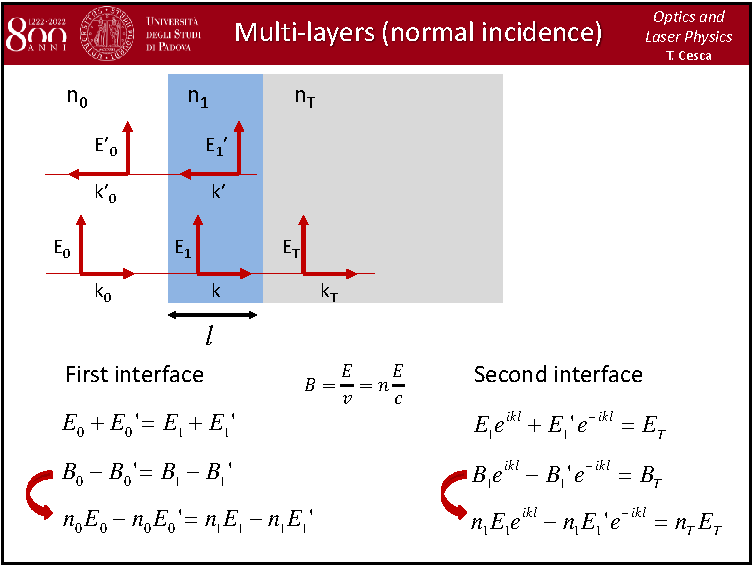
\includegraphics[page=1,width=1\textwidth]{../lessons/pdf_file/06_lecture.pdf}
\end{minipage}
\hspace{0.3cm}\vspace{0.3cm}
\begin{minipage}[c]{0.47\linewidth}

We shine a beam on a thin film of material. We can use this configuration in order to realize coatings with high reflectivity.

Let us consider normal incidence (TE and TM are degenerate). The substrate has a semiinfinite length.

Light is coming from left with electric field \( E_0 \) (the magnetic field coming out from the screen). We have the reflected wave \( E_0' \).
Inside the layer, we have the forward wave \( E_1 \) and the backward (reflected) which is \( E_1' \). We have the trasmitted wave \( E_T \).

This is an interference problem: how to imagine the interference of the wave forawrd and backward inside the layer.
Instead of inference, we can use the cointinuity equations for the tangentials components of electric and magnetic field at the interface.

\end{minipage}

For the second interface, we have to consider the propagation of the wave inside \( n_1 \). This is the solution of the problem in the steady state (we have a large number of cycles, interference of multiple waves until we reach a steady state solution, results independent on time).

In the end, we end up with four equations.

\subsubsection*{Slide 2}

\begin{minipage}[]{0.5\linewidth}
\centering
\includegraphics[page=2,width=1\textwidth]{../lessons/pdf_file/06_lecture.pdf}
\end{minipage}
\hspace{0.3cm}\vspace{0.3cm}
\begin{minipage}[c]{0.47\linewidth}

It is possible to simply this problem, instead of considering the amplitudes, we can consider the reflection and trasmission coefficients.

We rewrite the system in a matrix formulation. \( M \) is the \textbf{transfer matrix}.

In this framework the reflectivity is \( R= \abs{r}^2  \)and the transmittance \( T = \abs{t}^2  \). With this assumption:
\begin{equation*}
  R + \frac{n_T}{n_0} T \equiv 1
\end{equation*}
This convention is used for multi-layers typically.

\end{minipage}

\subsubsection*{Slide 3}

\begin{minipage}[]{0.5\linewidth}
\centering
\includegraphics[page=3,width=1\textwidth]{../lessons/pdf_file/06_lecture.pdf}
\end{minipage}
\hspace{0.3cm}\vspace{0.3cm}
\begin{minipage}[c]{0.47\linewidth}

Let us see how we can use this matrix formulation. Let us imagine to have a stack of different layers with different \( n \) with different thickness. The propagation vector inside each layer is related to the refractive index.

The transfer matrix is given by the product of the transfer matrix of each layer!

The order in which you have to multiply the matrix is important, but in this case you have to multiply the matrix from left (first illuminated layer) to right. This is the \textbf{main difference} with the Jones's notation.

\end{minipage}

\newpage

\subsubsection*{Slide 4}

\begin{minipage}[]{0.5\linewidth}
\centering
\includegraphics[page=4,width=1\textwidth]{../lessons/pdf_file/06_lecture.pdf}
\end{minipage}
\hspace{0.3cm}\vspace{0.3cm}
\begin{minipage}[c]{0.47\linewidth}

If we solve the system, the results for the reflection and trasmission coefficients are shown in this slide.

In many books, \( n_0 \) (environment) is assumed to be 1.

\end{minipage}

\subsubsection*{Slide 5}

\begin{minipage}[]{0.5\linewidth}
\centering
\includegraphics[page=5,width=1\textwidth]{../lessons/pdf_file/06_lecture.pdf}
\end{minipage}
\hspace{0.3cm}\vspace{0.3cm}
\begin{minipage}[c]{0.47\linewidth}

Let us see some examples of the above formulation.

Let us determine the reflectivity for a single layer embedded in an environment with \( n_0 \) and in a substrate of \( n_T \). \( \lambda  \) is the wavelength of the wave inside \( n_1 \).

The results in this slide for the reflectance are valid only for \( k l = \frac{\pi }{2} \).

Let us imagine that we want to obtain an \textbf{anti-reflection} coating. The condiction is that \( \sqrt{n_T n_0} = n_1  \).

In reality, you cannot get materials of any refractive index. First, the material should be transparent, easily deposited, durable... There are a lot of technological problems. For this problem, typically, for making an anti-reflection coating for glass we use $\text{MgF}_2$.
We can get a good value, which is not exactly zero but is very near.

\end{minipage}

\subsubsection*{Slide 6}

\begin{minipage}[]{0.5\linewidth}
\centering
\includegraphics[page=6,width=1\textwidth]{../lessons/pdf_file/06_lecture.pdf}
\end{minipage}
\hspace{0.3cm}\vspace{0.3cm}
\begin{minipage}[c]{0.47\linewidth}



\end{minipage}

\newpage

\subsubsection*{Slide 7}

\begin{minipage}[]{0.5\linewidth}
\centering
\includegraphics[page=7,width=1\textwidth]{../lessons/pdf_file/06_lecture.pdf}
\end{minipage}
\hspace{0.3cm}\vspace{0.3cm}
\begin{minipage}[c]{0.47\linewidth}

Let us imagine to have two layers with thickness again \( l = \lambda /4 \).

This is the reflectance of two layers with this thickness.

We get again the condition of anti-reflection.

\end{minipage}

\subsubsection*{Slide 8}

\begin{minipage}[]{0.5\linewidth}
\centering
\includegraphics[page=8,width=1\textwidth]{../lessons/pdf_file/06_lecture.pdf}
\end{minipage}
\hspace{0.3cm}\vspace{0.3cm}
\begin{minipage}[c]{0.47\linewidth}

This is an example graph of anti-relfection coating. We have a single layer of magnesium floride. The red curve is the one we should consider (normal incidence).

\end{minipage}

\subsubsection*{Slide 9}

\begin{minipage}[]{0.5\linewidth}
\centering
\includegraphics[page=9,width=1\textwidth]{../lessons/pdf_file/06_lecture.pdf}
\end{minipage}
\hspace{0.3cm}\vspace{0.3cm}
\begin{minipage}[c]{0.47\linewidth}

This approach could be applied to determine high reflectance coatings (mirror).

We have a substrate \( n_T \), environment \( n_0 \) and a stack of \( 2 N \) layers of two different materials with \( n_H \) (high) and \( n_L \) (low) and with \( l = \lambda /4 \).

When \( N \rightarrow \infty  \) we obtain \( R \rightarrow 1 \)!

\end{minipage}

\subsubsection*{Slide 10}

\begin{minipage}[]{0.5\linewidth}
\centering
\includegraphics[page=10,width=1\textwidth]{../lessons/pdf_file/06_lecture.pdf}
\end{minipage}
\hspace{0.3cm}\vspace{0.3cm}
\begin{minipage}[c]{0.47\linewidth}

This is a practical example.

If the number of layer is very large, the order of \( n_H \) and \( n_L \) does not play an important role. Instead, in different cases, the order is important and it makes a different.

\end{minipage}

\subsubsection*{Slide 11}

\begin{minipage}[]{0.5\linewidth}
\centering
\includegraphics[page=11,width=1\textwidth]{../lessons/pdf_file/06_lecture.pdf}
\end{minipage}
\hspace{0.3cm}\vspace{0.3cm}
\begin{minipage}[c]{0.47\linewidth}

This is the reflectance for a stack of \( \text{TiO}_2 \).

The dashed line gives the spectral trend for three couples. You obtain a reflectivity of around \( 60 \% \). If you increase the number of layers, you obtain \( 100 \% \).

We are consider an interference problem, so we have interference effects (oscillation in the reflectivity).

\end{minipage}

\subsubsection*{Slide 12}

\begin{minipage}[]{0.5\linewidth}
\centering
\includegraphics[page=12,width=1\textwidth]{../lessons/pdf_file/06_lecture.pdf}
\end{minipage}
\hspace{0.3cm}\vspace{0.3cm}
\begin{minipage}[c]{0.47\linewidth}

This happens every time you have a stack of a low and high refractive index

\end{minipage}

\subsubsection*{Slide 13}

\begin{minipage}[]{0.5\linewidth}
\centering
\includegraphics[page=13,width=1\textwidth]{../lessons/pdf_file/06_lecture.pdf}
\end{minipage}
\hspace{0.3cm}\vspace{0.3cm}
\begin{minipage}[c]{0.47\linewidth}

This can be solved if you make an \textbf{apodized}, you modulate the values of the refractive index, which means modulating the phase of your wave inside the layers. You can play with this and find the configuration which reduces the oscillation in the border and give you high reflectivity.

\end{minipage}

\subsubsection*{Slide 14}

\begin{minipage}[]{0.5\linewidth}
\centering
\includegraphics[page=14,width=1\textwidth]{../lessons/pdf_file/06_lecture.pdf}
\end{minipage}
\hspace{0.3cm}\vspace{0.3cm}
\begin{minipage}[c]{0.47\linewidth}

How to move to a situation which is no more at normal incidence. In this case, we should distinguish TE and TM.

We have the environment \( n_0 \), the material \( n_1 \) and the substrate \( n_T \).

This is the solution of the problem. We consider the expression for \( r \) and \( t \) at normal incidence. We consider the transfer matrix. The tickness of the layer is \( z \). The argument of the cosine and sine is \( \beta = k \cos(\theta )z  \), where \( k \) is the modulus of the propagation vector within the layer, propagation angle within the layer \( \theta  \).

These are the substitution we have to do. Also the mapping of the conservation of energy is changed.

\end{minipage}

\subsubsection*{Slide 15}

\begin{minipage}[]{0.5\linewidth}
\centering
\includegraphics[page=15,width=1\textwidth]{../lessons/pdf_file/06_lecture.pdf}
\includegraphics[page=16,width=1\textwidth]{../lessons/pdf_file/06_lecture.pdf}
\end{minipage}
\hspace{0.3cm}\vspace{0.3cm}
\begin{minipage}[c]{0.47\linewidth}

This is the case for TM.

The important point is that from normal incidence to oblique incidence you have to distinguish between TE and TM. 

\end{minipage}






\end{document}
